\capitulo{5}{Aspectos relevantes del desarrollo del proyecto}

En este apartado se recogen los aspectos más importantes. Explicando las decisiones tomadas del proyecto, y las consecuencias que suponen, comentando los errores y como se solucionaron.

\section{Inicio}

Una vez se me explicó la idea que se buscaba con este proyecto, me gustó la idea de poder hacer una aplicación que pudiera servir al sistema sanitario público.

En este inicio, empecé a imaginarme como podría ser la aplicación haciendo bocetos mentales de las interfaces, como era muy efímero, se hizo una búsqueda de aplicaciones similares, donde se encontró la aplicación Ret-iN CaM. Con una idea más formada, se hicieron los bocetos iniciales de la aplicación.

\section{Metodologías}

Como ya se ha comentado anteriormente, se decidió utilizar una metodología SCRUM, no siguiéndose al completo, puesto que los equipos de desarrollo en esta metodología están compuesto de 3 a 9 personas, a su vez, hay reuniones que no se han podido realizar, entre otras cosas. Pero, con esta metodología se ha buscado que el proyecto tuviese una metodología ágil.

Un fallo cometido con respecto esta metodología ha sido que los martes cambiaba de sprint a las 8 de la mañana, y la revisión para finalizar el sprint, se realizaba los martes por la mañana, haciendo que algunas veces las tareas cambiasen de sprint cuando no debían, y por tanto, la reunión para comenzar el sprint se realizaba con el sprint comenzado.

Las características ágiles de este proyecto son:
\begin{itemize}
    \item Los sprints planeados han tenido una duración de 2 semanas, entregando un incremento al final de cada uno.
    \item Se han realizado reuniones, tanto para finalizar el sprint, como para el inicio del siguiente, teniendo en consideración el fallo comentado anteriormente.
    \item Las tareas que se planeaban para un sprint, se estimaban y priorizaban en un tablero Kanban, tanto físicamente como con la herramienta ZenHub. Aunque con el paso de los sprints, se dejo de hacer físicamente.
    \item Para comprobar el progreso del proyecto, se ha utilizado los gráficos burndown, que aunque los ofrece ZenHub, se han realizado a mano, por el fallo comentado.
\end{itemize}

Al principio del proyecto se planeaba utilizar otras metodologías como \textit{Test-Driven-Development} o como \textit{Data-driven testing}, junto con pruebas automáticas, vistas durante el año académico en la asignatura Validación y pruebas, para comprobar como las implementaciones que se iban realizando en el proyecto no se veían afectadas entre ellas y que se implementaban correctamente. 

Pero al implementar las distintas interfaces, se decidió hacer pruebas manuales, las cuales proporcionan una mayor comprensión de la interacción que tiene el usuario con la aplicación, buscando siempre que el usuario entienda el sistema.

\section{Formación}

Para el proyecto no fue necesario el aprendizaje de un nuevo lenguaje, puesto que para la aplicación de Android Studio se usó el lenguaje Java, visto durante la carrera y para la creación de la red neuronal se usó el lenguaje Python, que también se ha visto. 

Pero, sí que ha sido necesario el uso de tutoriales, guías tanto de Android Studio y como keras y tensorflow para implementar correctamente el código.

Para la utilización de la red VGG-16, se leyó el articulo: \textit{Very Deep Convolutional Networks for Large-Scale Image Recognition}(Karen Simonyan y Andrew Zisserman) \cite{simonyan2015deep}.

Además han surgido otros errores, tanto de programación, como de incompatibilidad entre otras cosas; que fueron solucionados por la comunidad de stackoverflow y de YouTube.


\section{Conjunto de datos}

El conjunto de datos utilizado para la creación del modelo, es un conjunto de datos real, lo que significa que las imágenes no se han creado ni artificialmente; normalmente esta idea se asocia a ensayos clínicos aleatorios, donde primero se desidentifica la imagen obtenida del paciente.

Existen varios problemas debido al conjunto de datos real, entre ellos, se han observado el desbalanceo de datos, que es debido a que hay una disparidad en la cantidad de imágenes de un tipo y de otro, esto puede producir que el modelo cree patrones donde no los hay.
Otro problema, es la calidad de la imagen, debido a que estas imágenes no tienen porque realizarse en el mismo hospital, puede haber variaciones en el procedimiento del retinógrafo.

En la figura \ref{fig:imagenes con calidad mala} se pueden observar imágenes del dataset con una calidad mala, ya sea porque se ha realizado mal la retinografía, o porque el retinógrafo fuese defectuoso.

        \begin{figure}[!ht]
                 \centering
                 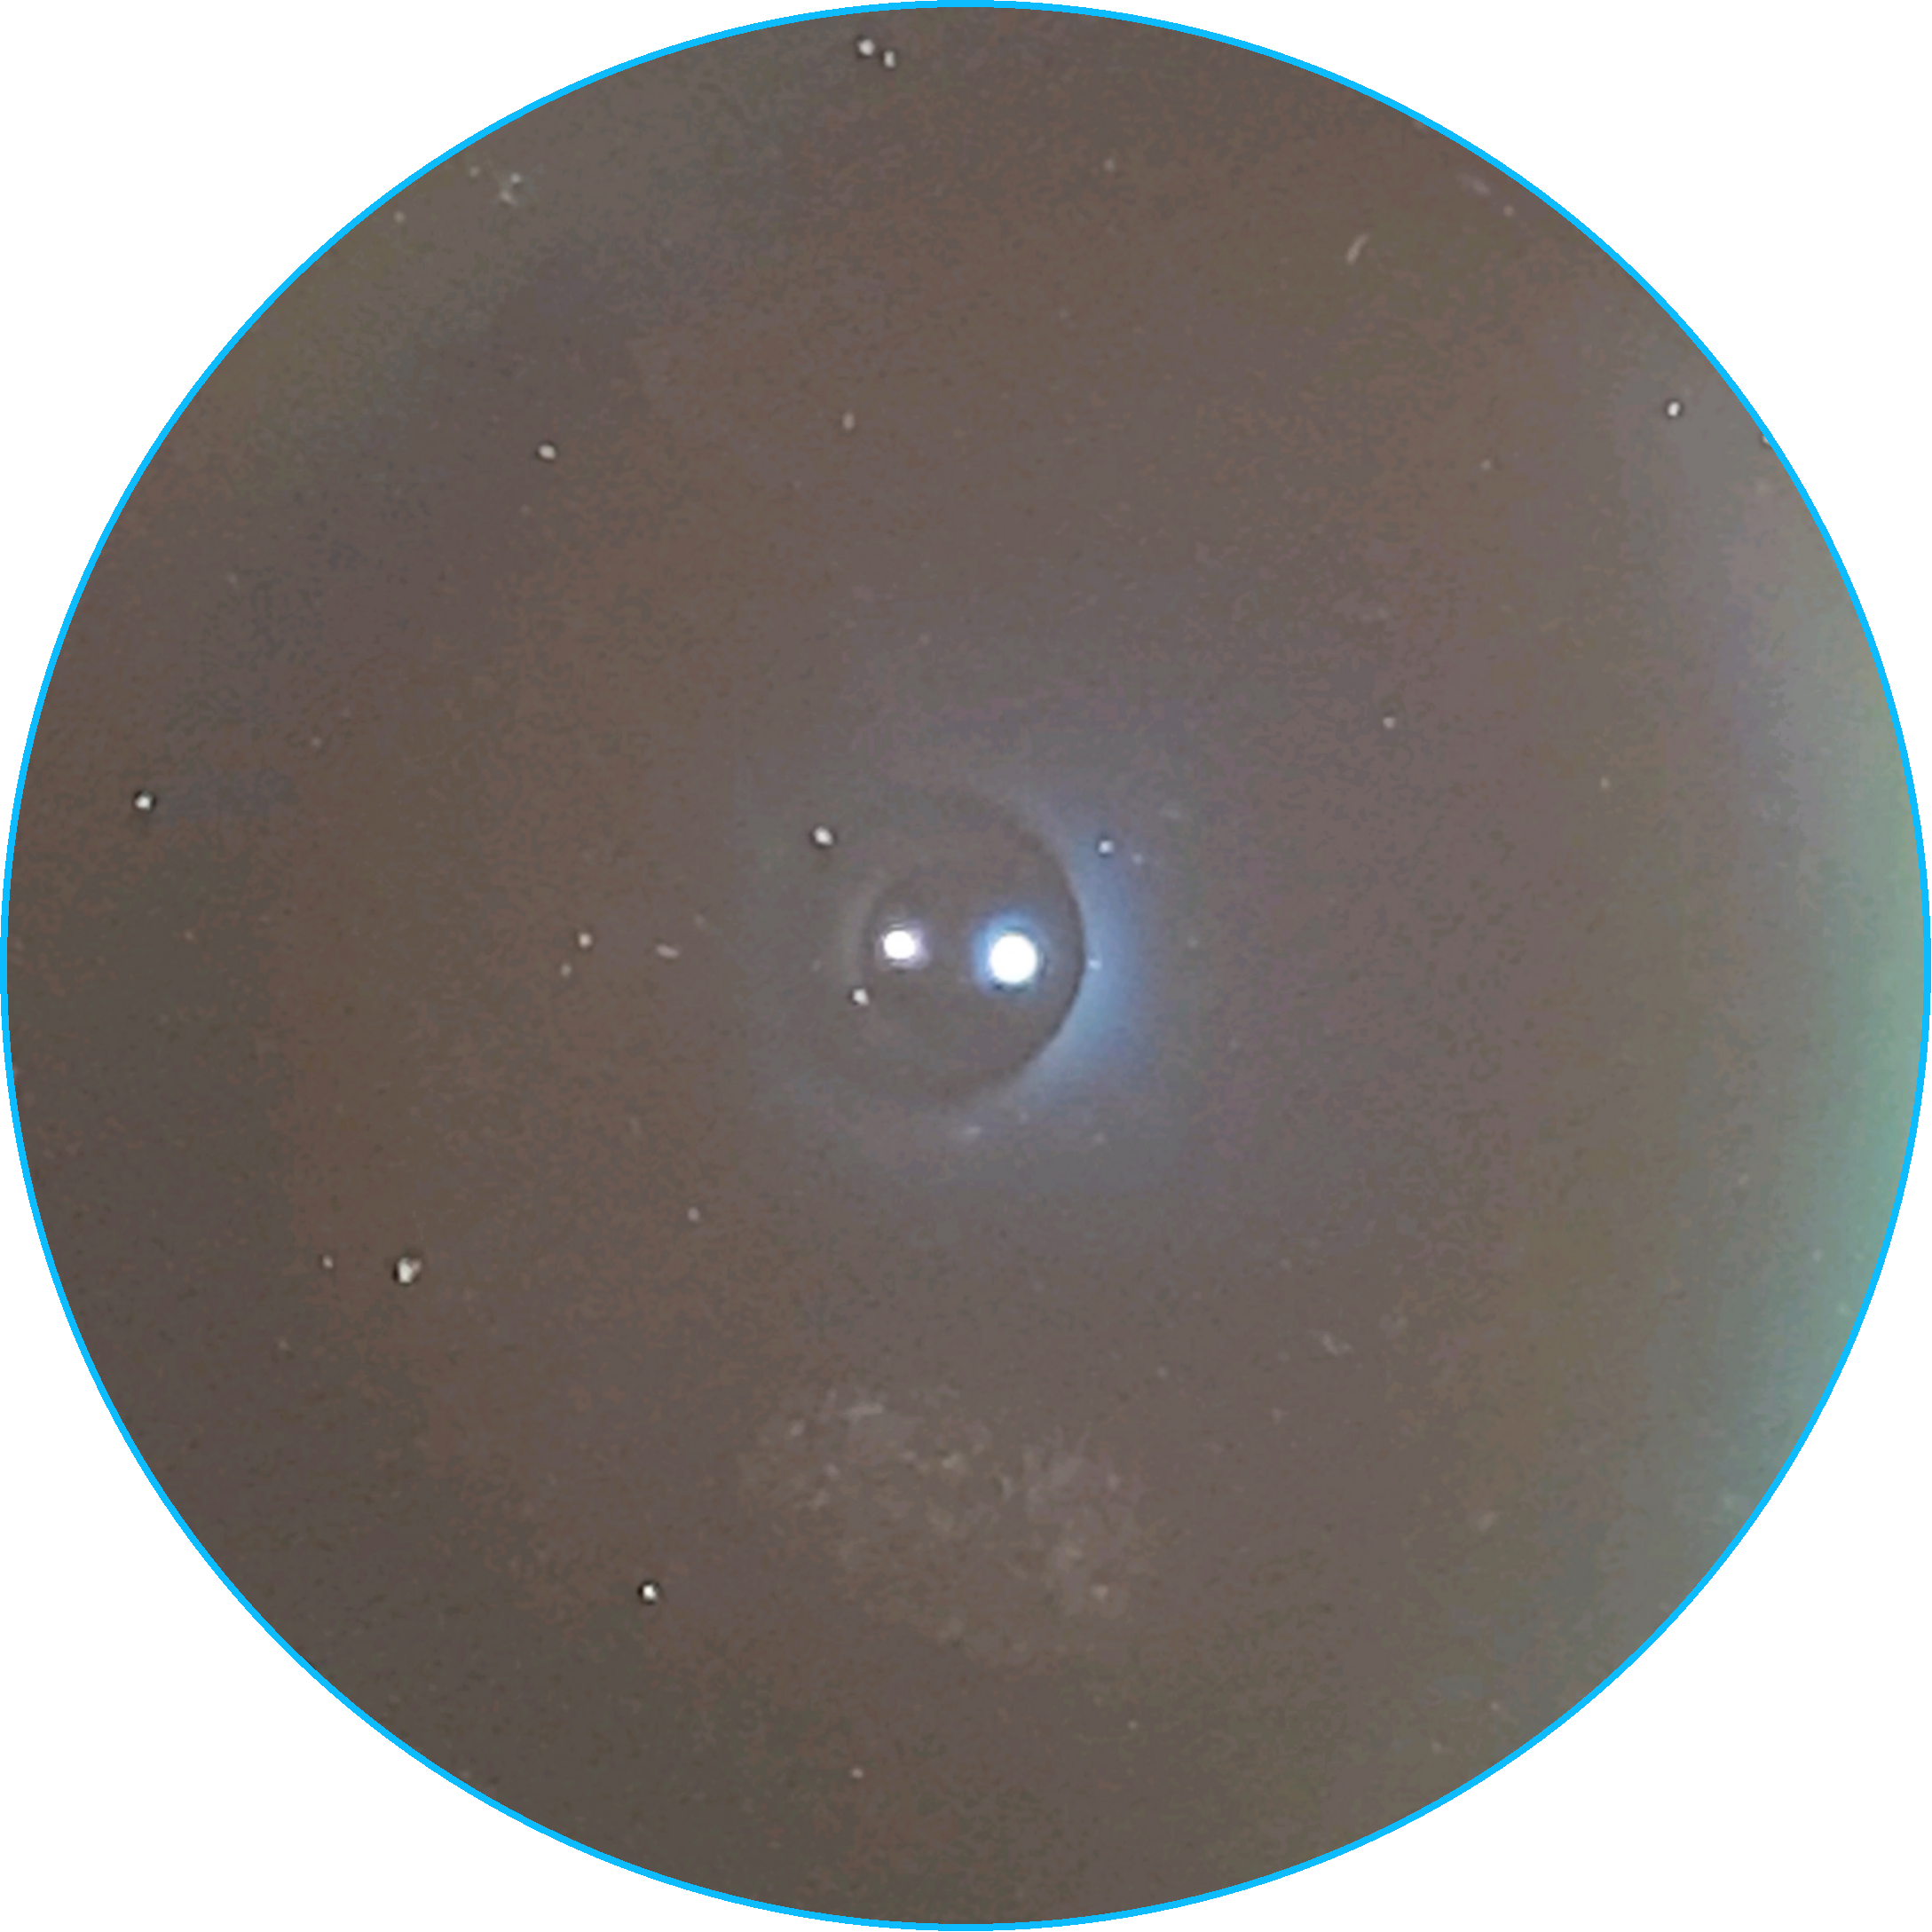
\includegraphics[width=0.45\textwidth]{img/dataset/315483GD.png}
                 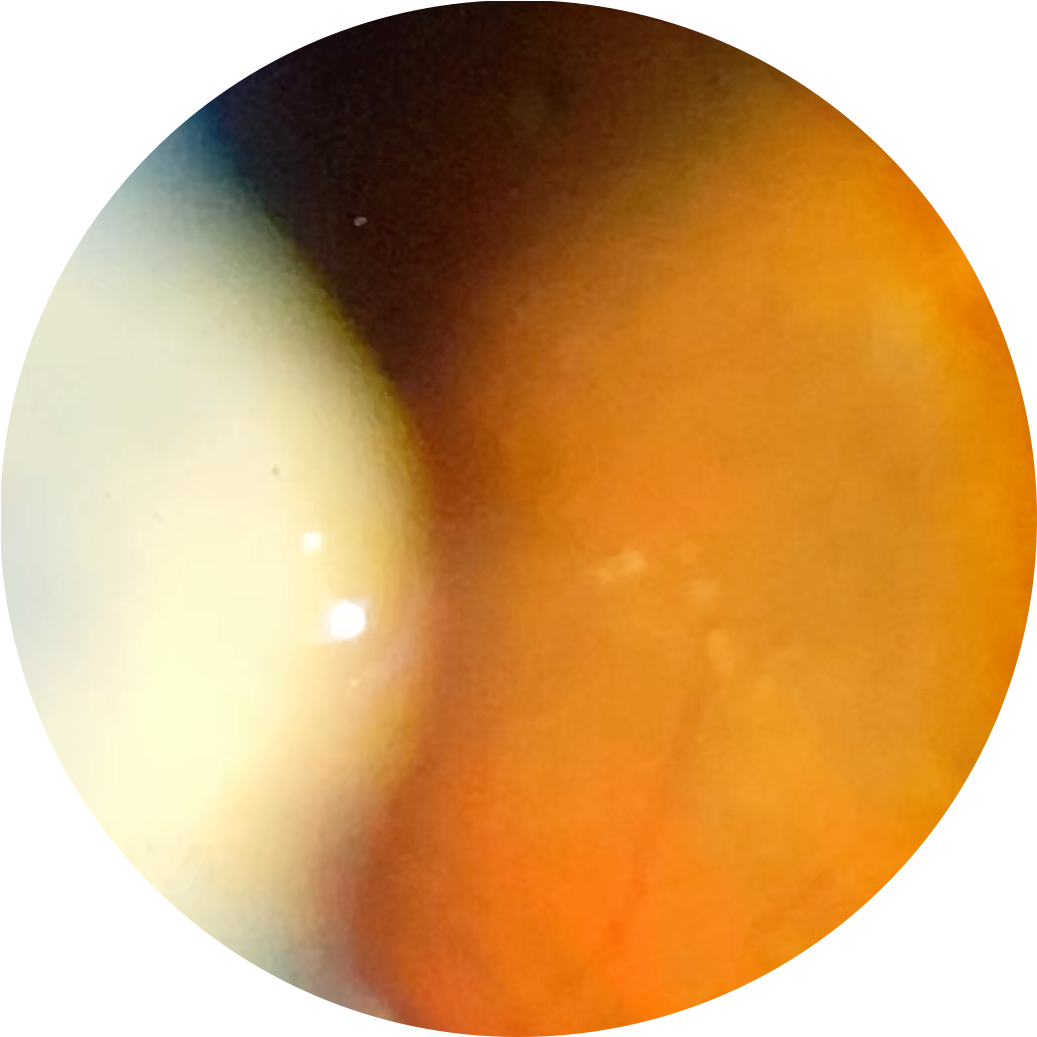
\includegraphics[width=0.45\textwidth]{img/dataset/365017ED.PNG}
                  \caption{Imágenes con una calidad mala}
                 \label{fig:imagenes con calidad mala}
        \end{figure}

Por otro lado, en la figura \ref{fig:imagenes con calidad buena} se pueden observar imágenes de buena calidad. Donde en la imagen de la izquierda, el paciente tiene un grado alto de retinopatía diabética y la imagen de la derecha no tiene ningún grado.

\begin{figure}[!ht]
    \centering
    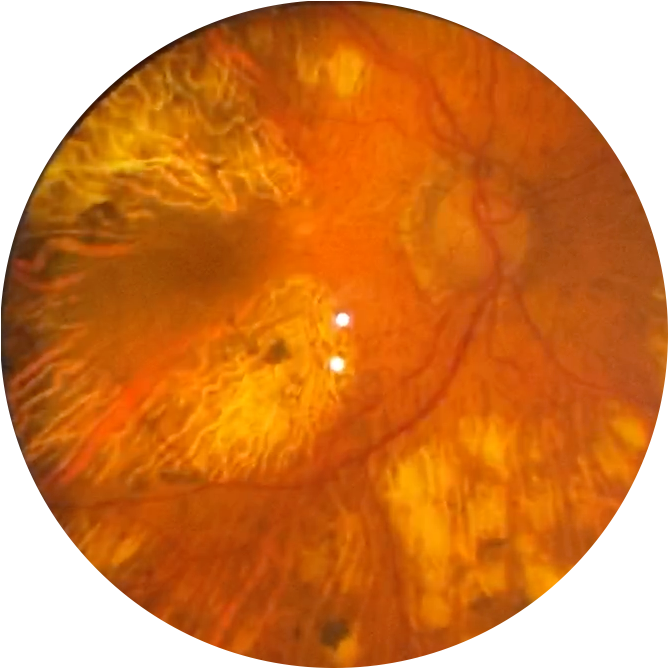
\includegraphics[width=0.45\textwidth]{img/dataset/517191ED.PNG}
    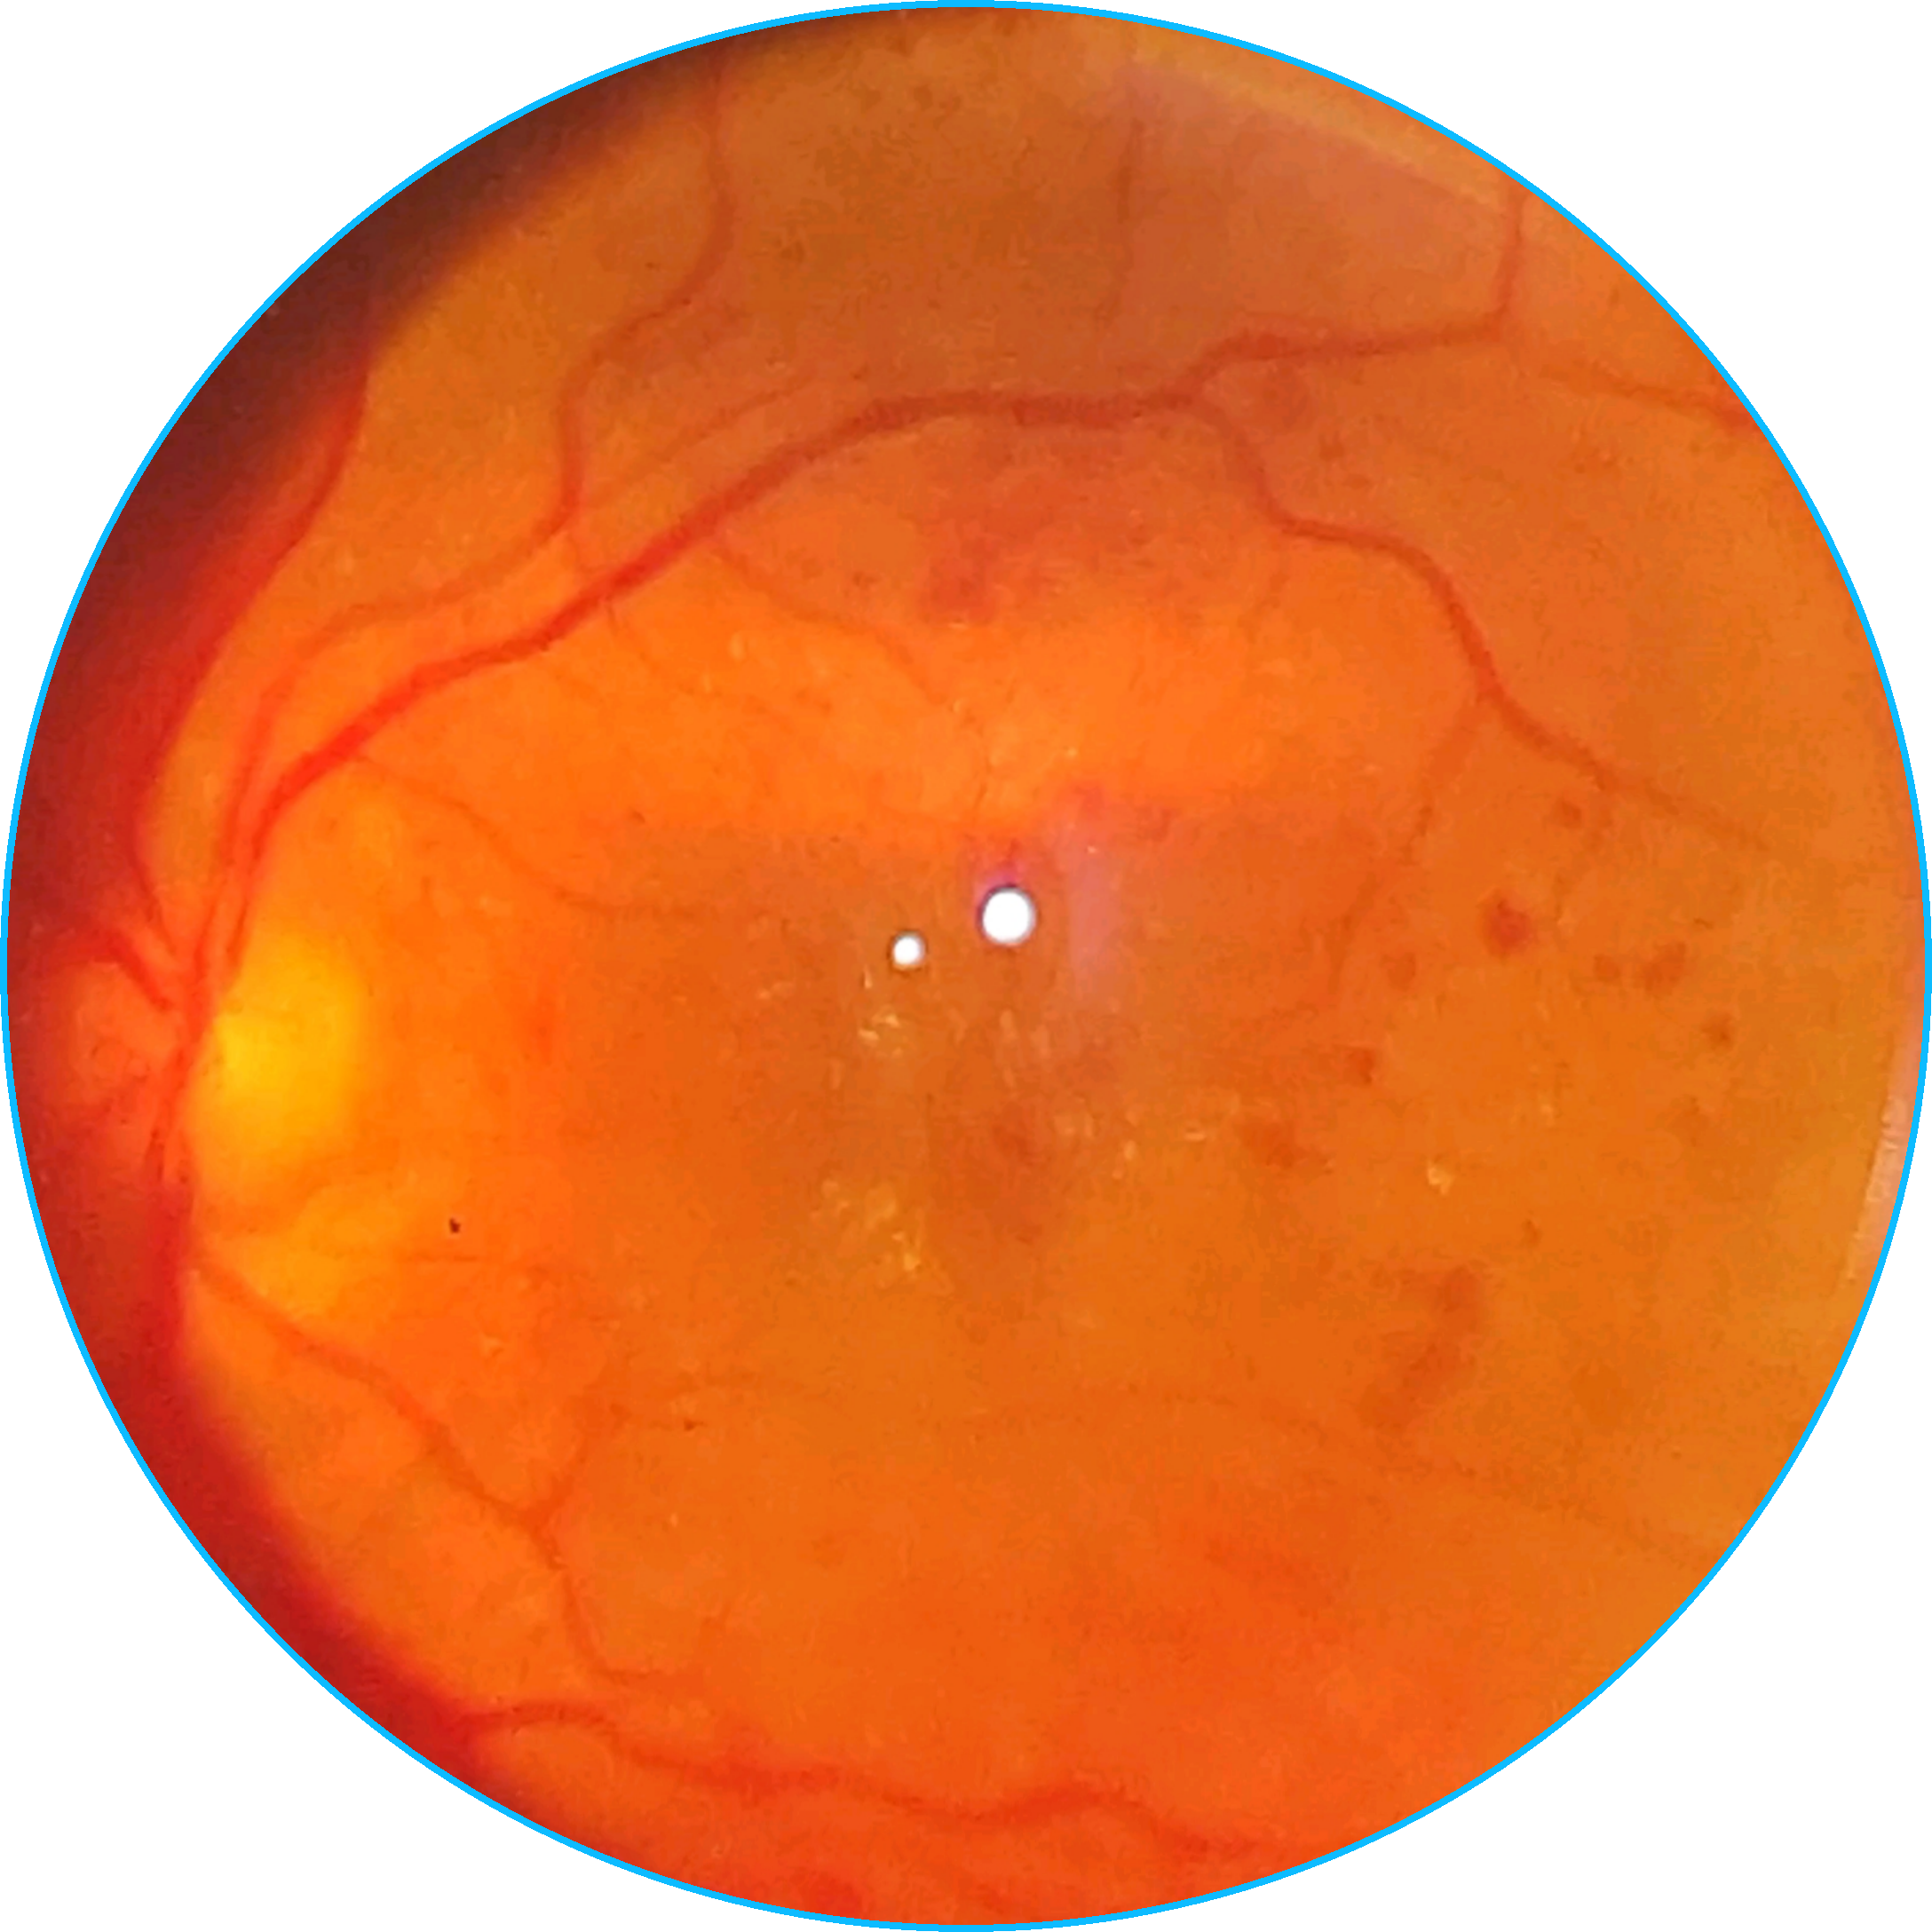
\includegraphics[width=0.45\textwidth]{img/dataset/442507GI.png}
    \caption{Imágenes con una calidad buena}
    \label{fig:imagenes con calidad buena}
\end{figure}

\section{Creación del modelo para detectar la calidad de imagen}

Para crear un modelo keras en python, se usó la guía que viene en TensorFlow para \href{https://www.tensorflow.org/tutorials/images/classification?hl=es-419}{clasificación de imágenes}\cite{tensorflow-classification-tutorial} utilizando un modelo VGG-16.

El conjunto de datos se divide en 2 partes, el conjunto de imágenes, y un csv con el nombre de la imagen y la calidad que tiene esta.
La calidad esta compuesto de números del 1 al 5, y se considera una calidad aceptable cuando el valor es 4 o 5, y no es aceptable cuando es menor que 4. 
Para definir el conjunto de entrenamiento, de test y de validación se dividió el conjunto de datos de forma 80\% para entrenar, 10\% de test y el otro 10\% validación.

Como métricas utilizadas, se empezó utilizando la \textit{accuracy}, la cual mide el número de aciertos totales entre el número total de ejemplares. Como se ha comentado en el apartado de Conceptos teóricos, esta medida no es recomendable para datos desbalanceado.

Por ello se usan las medidas precisión y recall. Para comprobar que modelo es mejor, se ha representado la matriz de confusión y se ha calculado el f1-score, el cual se ha introducido en el nombre del modelo creado.

Como el modelo creado puede variar según el conjunto de entrenamiento escogido, se ha ejecutado varias veces para obtener el mejor resultado posible; otro valor a tener en cuenta en la creación del modelo es la tasa de aprendizaje. Una tasa de aprendizaje baja suele hacer que el modelo no se ajuste lo suficiente al resultado esperado; y una tasa de aprendizaje demasiado alta, puede producir que el modelo aprenda los datos. En la imagen \ref{fig:overfiting}, se puede observar el sobreajuste y el infrajuste, que son los resultados posibles al escoger una tasa de aprendizaje alta o baja.
        \begin{figure}[!ht]
                 \centering
                 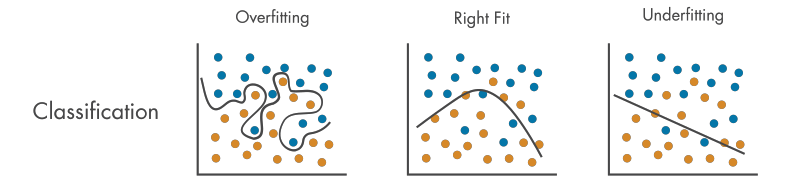
\includegraphics[width=0.9\textwidth]{img/overfiting-underfiting.png}
                  \caption{Comparación de sobreajuste e infrajuste. Imagen adaptada de \cite{mathworks-overfitting}}
                 \label{fig:overfiting}
        \end{figure}

Además, en un principio, se quería clasificación binaria con clasificación multiclase. Cuando se compararon estos valores, se utilizaba la medida ``accuracy'', que como ya se ha explicado no es recomendable en clasificación binaria. Durante la integración de la matriz de confusión en la clasificación multiclase, no se logró una buena visualización, y por ello no se hizo esta comparación con F1-Score.

En la gráfica \ref{fig:accuracy}, se observa el historial del mejor caso observado para la clasificación binaria.

        \begin{figure}[!ht]
                 \centering
                 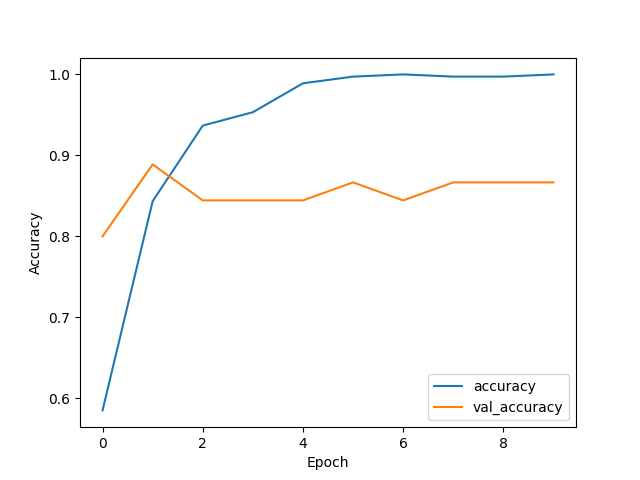
\includegraphics[width=0.5\textwidth]{img/modelo2-0.009int2_0.913043498992919920230525-172156.png}
                  \caption{Historial de la evolución de la ``accuracy''  de un modelo cuyo resultado de test era de 91\% }
                 \label{fig:accuracy}
        \end{figure}


Al observar las matrices de confusión obtenidas, había 2 resultados mejores que los demás, y en varios casos, se obtuvo el resultado mencionado anteriormente, donde el modelo indicaba que todas las imágenes eran validas, pero en este caso, no se calculaba la ``accuracy''.

En la figura \ref{fig:comparacion de modelos}, se puede observar como y la matriz inferior, hace referencia al caso comentado, y las 2 matrices de confusión de la parte superior, hacen referencia a 2 modelos que clasifican de forma correcta casi todos los datos de test.

Para la matriz de la izquierda:
\begin{center}
    $Precision = \dfrac{11} {11 + 2} = 0.85 $

    $Recall = \dfrac{11} {11 + 0} = 1 $

    $F_1 = 2 \dfrac{0.85 * 1} {0.85 + 1} = 0.9189 $
\end{center}


Para la matriz de la derecha:
\begin{center}
    $Precision = \dfrac{10} {10 + 1} = 0.909 $

    $Recall = \dfrac{10} {10 + 1} = 0.909 $

    $F_1 = 2 \dfrac{0.909 * 0.909} {0.909 + 0.909} = 0.909 $    
\end{center}

Para la matriz de abajo:

\begin{center}
    $Precision = \dfrac{0} {0 + 0} = NaN $

    $Recall = \dfrac{0} {0 + 11} = 0 $

    $F_1 = 2 \dfrac{NaN * 0.909} {NaN + 0.909} = NaN $    
\end{center}

Entre las 2 opciones de la figura, aunque ambas han tenido la misma cantidad de aciertos, según la formula del f1-score, el modelo de la izquierda es mejor, puesto que acierta correctamente en todos los que predice como APTO, cosa que el modelo de la derecha no hace.

        \begin{figure}[!ht]
                 \centering
                 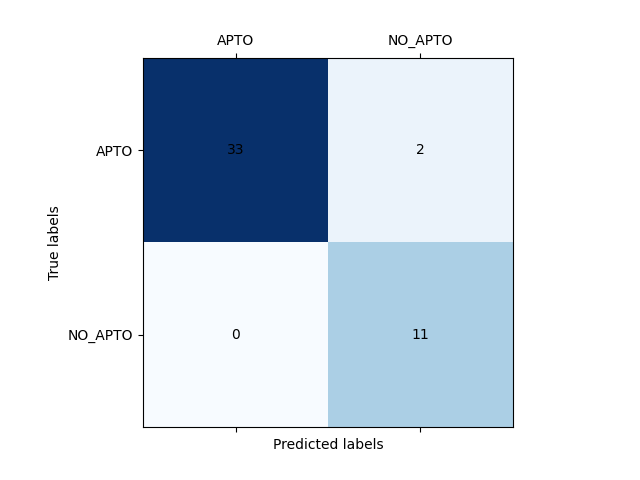
\includegraphics[width=0.45\textwidth]{img/modelo2-0.003int2_0.9166666720476415_20230603-003149.png}
                 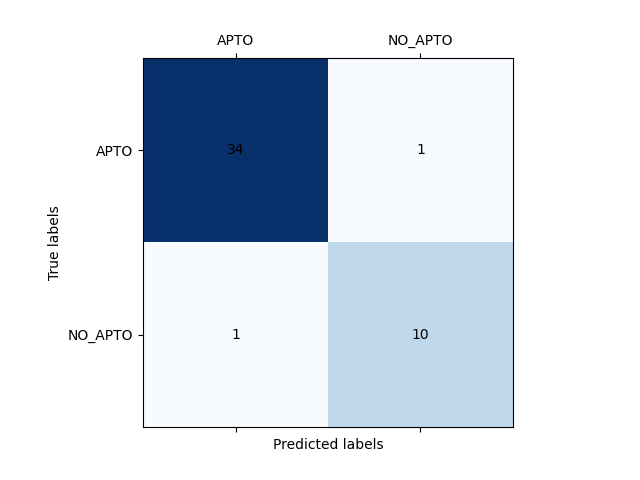
\includegraphics[width=0.45\textwidth]{img/modelo2-0.005int2_0.9090909361839294_20230603-010653.png}
                 \centering
                 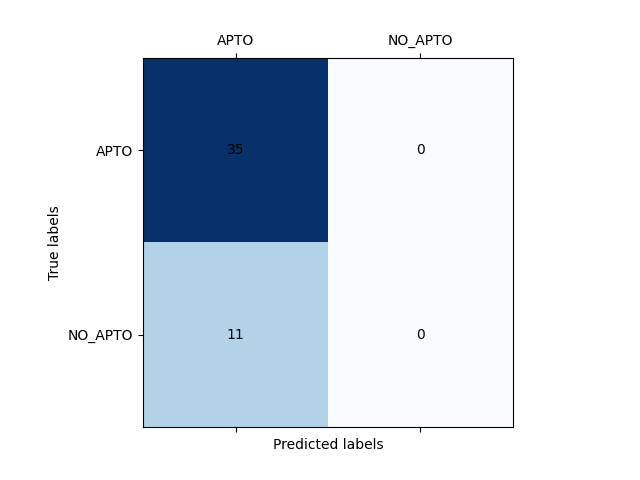
\includegraphics[width=0.45\textwidth]{img/modelo2-0.002int1_0_20230610-154306.png}
                  \caption{Comparación de los modelos destacables}
                 \label{fig:comparacion de modelos}
        \end{figure}


\section{Aplicación Android}

Para trabajar en el proyecto, se pensó en utilizar Android Studio o UNITY, la opción seleccionada fue Android Studio, porque ya se tenían nociones previas. 

Con el IDE seleccionado, se tenía que crear un proyecto, donde se seleccionó como API la versión 21, que como informa Android Studio, se puede ejecutar en el 99,5\% de dispositivos \ref{fig:API-Android}.

        \begin{figure}[!ht]
                 \centering
                 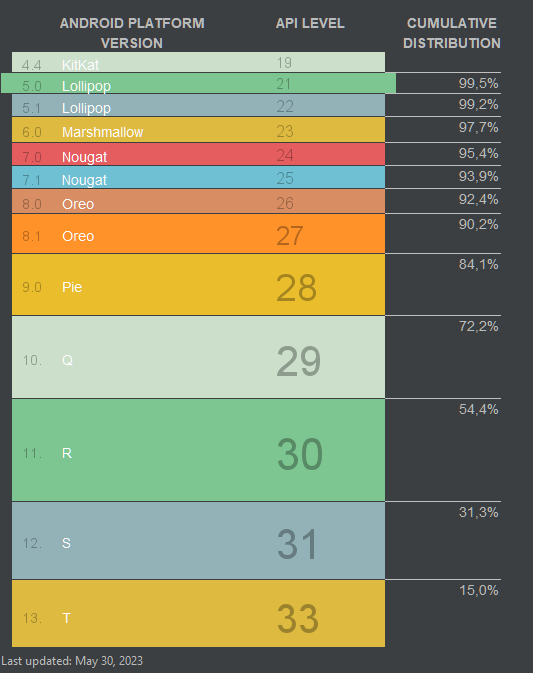
\includegraphics[width=0.45\textwidth]{img/API-android.png}
                  \caption{Porcentaje de dispositivos según la API. Imagen obtenida de Android Studio.}
                 \label{fig:API-Android}
        \end{figure}

Después de terminar el boceto igual al realizado manualmente,(\href{https://github.com/mfg1014/Retinopatia-diabetica/issues/7}{Issue \#7}), se realizaron cambios en la interfaz, añadiendo un modo oscuro, la posibilidad de entrar como invitado, una red neuronal que determine la calidad de la imagen, y en caso de ser mala, se repita la imagen, y una opción para cambiar el orden de los ojos, permitiendo que el médico elija su propia preferencia. Estas funcionalidades han sido introducidas en Issues posteriores.

Durante la implementación se encontraron varios bugs, que en algunos casos se encontraban durante la programación de esas partes del código, y en otros casos, se encontraban durante la ejecución de la aplicación de forma normal. De esta forma, en algunos casos se programaron Issues orientadas a la eliminación de estos errores, y en otros casos se hizo sobre la propia Issue que se estaba introduciendo.

Entre los bugs encontrados, cabe destacar los siguientes:
\begin{itemize}
    \item Bug con el modo oscuro entre actividades, al introducir la variable que indicaba que el usuario había activado el modo oscuro, al pasar la variable de una actividad a otra, en algunos lugares estaba mal instanciada y producía errores de ejecución.
    \item Bug con el modo oscuro de texto e imágenes no legibles, cuando se añadió el modo oscuro, algunas vistas de la interfaz no se cambiaron de forma correcta, de forma que el color del fondo no se distinguía de la vista.
    \item Bug con el botón que cambia el orden de los ojos, durante la implementación de esa parte, solo se probó si el botón cambiaba el orden de forma correcta, y así era, pero cada vez que se entraba a esa ventana estaba siempre en la misma posición. 

    \item Bug con LocalDateTime, al principio para introducir en la base de datos la fecha del informe introducido o la fecha de nacimiento de los médicos y los pacientes, se utilizaba la clase LocalDateTime, aunque Android Studio avisaba de que era recomendable no usar esa clase, se utilizó, el problema surgió cuando se probó con un Android con versión API inferior, donde ni inicializaba la aplicación.

    \item Bug con la base de datos, la primera base de datos, era un conjunto de clases java donde con un constructor se inicializaban los usuarios, pacientes, informes,... El problema surgió cuando cada vez que se inicializaba la aplicación se usaba el constructor. Se implementó el patrón singleton y seguía ocurriendo el mismo problema, por ese motivo, se decidió utilizar SQLite para la base de datos.

    \item Bug con la petición de permisos, en la forma que se pedían los permisos, creaba infinitas comprobaciones de los permisos de cámara, haciendo que si no se contestaba durante un tiempo, la aplicación ``crasheará''. Se solucionó eliminando el bucle y pidiendo un sólo permiso a la vez. 
\end{itemize}

\subsection{Cámara en Android Studio}

La primera implementación en la que se necesito una guía, fue en el uso de la cámara en una aplicación, guardando posteriormente la imagen obtenida.

Para ello, primero se necesitaba inicializar la cámara, que se obtuvo una referencia de la propia página de  Android \cite{android-camera-intents}.

Una vez implementado, surgió un problema debido a los permisos de la aplicación, puesto que no se abría la cámara. Buscando como implementar la petición de los permisos de la cámara durante la ejecución; esta referencia también se obtuvo de la propia Android \cite{android-permissions-requesting}.

Ya abierta la cámara, se tenía que guardar la imagen realizada, puesto que se hacia la foto, pero no se mostraba al usuario ni se guardaba de forma interna. Llegando otra vez a la página de Android, donde en un ejemplo se podía ver como se implementaba \cite{android-intents-result}. 

Con la imagen obtenida de forma local, solo había que mostrarla al usuario tarea que ya se sabía realizar.

\subsection{Galería en Android Studio}

Al igual que en la cámara, no se tenían los conocimientos para implementar este requisito, pero como la cámara se implementó anteriormente, se utilizó el mismo enlace para obtener la imagen seleccionada. \cite{android-intents-result}. 

Para llamar a esta actividad, se usó la respuesta de un foro de \href{https://stackoverflow.com/questions/38352148/get-image-from-the-gallery-and-show-in-imageview}{stackoverflow} \cite{stackoverflow-gallery-imageview}, que permitió llamar de forma correcta a esta actividad.

Como en el caso de la cámara, se pensó que también sería necesario el uso del permiso para leer almacenamiento externo. Surgiendo un error de ejecución. Se pensó que era un error de programación hasta que se encontró que a partir de la API 30, el permiso para leer almacenamiento externo no es necesario \cite{android-storage-privacy}.

\subsection{Implementación de las redes neuronales usando TensorFlow Lite}

 Para integrar las redes neuronales se recomiendan implementar en formato TensorFlow Lite, por lo que era necesario una conversión del modelo, puesto que inicialmente tenían formato keras. Por lo que para integrar las redes neuronales se buscó información de las siguientes páginas:
\begin{itemize}
    \item Cargar un modelo TensorFlow Lite en Android \cite{tensorflow-lite-android-quickstart}
    \item Convertir modelo keras en modelo TensorFlow js \cite{tensorflow-js-import-keras}. Con esta idea, se usó la idea para convertir en formato TensorFlow Lite.
    \item Crear objeto Interprete \cite{tensorflow-lite-guide}.
    \item Preprocesamiento modelo VGG16~\cite{tensorflowVGG16}
    \item Preprocesamiento modelo ResNet50V2~\cite{tensorflowResNet50V2}
\end{itemize}

Con la información obtenida de los enlaces anteriores, se observo que para ejecutar un modelo era necesario abrir un Interprete con el cual se ejecuta el modelo, que es necesario hacer un conjunto de transformaciones .

Esta transformación de una cadena de texto a byteBuffer se hace de esta forma:
\lstset{
  language=Java,
  basicstyle=\footnotesize\ttfamily,
  keywordstyle=\color{blue},
  commentstyle=\color{green!60!black},
  stringstyle=\color{red},
  showstringspaces=false,
  breaklines=true,
  breakatwhitespace=true,
  tabsize=4,
  numbers=none,
  numberstyle=\tiny,
  frame=single,
  framexleftmargin=5mm,
  xleftmargin=5mm
}
\begin{lstlisting}
AssetFileDescriptor fileDescriptor = context.getAssets().openFd(fileName);
FileInputStream inputStream = new FileInputStream(fileDescriptor.getFileDescriptor());
FileChannel fileChannel = inputStream.getChannel();
long startOffset = fileDescriptor.getStartOffset();
long declaredLength = fileDescriptor.getDeclaredLength();
MappedByteBuffer mappedByteBuffer = fileChannel.map(FileChannel.MapMode.READ_ONLY, startOffset, declaredLength);
\end{lstlisting}

Con el modelo ya cargado, se necesita crear el \textit{input}, donde se encuentra la imagen preprocesada y el \textit{output}, que es una variable donde se guardan los resultados de la ejecución del modelo. El interprete se ejecuta con el comando run, junto con los atributos mencionados.

Para probar si el interprete funcionaba, se hizo un modelo básico que calculaba la operación XOR en la \href{https://github.com/mfg1014/Retinopatia-diabetica/issues/21}{Issue \#21}.

Posteriormente, se usó la red publicada por Lorenzo Baraldi~\cite{github-vgg16} para probar los resultados con imágenes. Para introducir esta red neuronal se necesita el preprocesamiento de los datos y para su ejecución se necesita saber el número de salidas de la red; esta red esta destinada a el conjunto de datos ``imagenet''~\cite{github-imagenet-classes} lo que significa que busca clasificar entre 1000 categorías distintas.
La issue relacionada a esta actividad, es \href{https://github.com/mfg1014/Retinopatia-diabetica/issues/24}{Issue \#24}.
Además, en esa tarea, se pensó que algunas redes neuronales tardan más de lo esperado en ejecutarse, y para que el usuario no tenga que esperar a que se termine de ejecutar, se implementó un hilo con las actividades de la red neuronal, permitiendo que se ejecute en segundo plano y se almacene el resultado en la base de datos.

Finalmente, se añadió la red entrenada para la clasificación de la retinopatía diabética, la cual es una red convolucional ResNet50v2. Añadiendo el preprocesamiento correspondiente. Esta Issue se corresponde con \href{https://github.com/mfg1014/Retinopatia-diabetica/issues/41}{Issue \#41}. Sufriendo pequeños cambios en futuras releases. 

Los resultados de esta red pueden ser:

\begin{itemize}
    \item 0 indica que el paciente tiene NPDR.
    \item 1 indica que el paciente tiene NPDR leve.
    \item 2 indica que el paciente tiene NPDR moderada.
    \item 3 indica que el paciente tiene NPDR severa.
    \item 4 indica que el paciente tiene PDR.
\end{itemize}

Por último, se añadió la red de calidad, la cual es una red convolucional VGG-16. Añadiendo su preprocesamiento correspondiente que ya se había realizado anteriormente. Esta Issue se corresponde con \href{https://github.com/mfg1014/Retinopatia-diabetica/issues/42}{Issue \#42}. Sufriendo pequeños cambios en futuras releases. 

Los resultados de esta red pueden ser:

\begin{itemize}
    \item 0 indica que la foto tiene una calidad mala.
    \item 1 indica que la foto tiene una calidad buena.

\end{itemize}